Materials contains a describtion of the given data of PFP subjects and which program is used to form the deep learning model to predict the duration of the PFP. 

\section{Data}
Data used in this project were collected beforehand. The data consists of pain maps which were drawn by subjects with PFP through the use of an application Navigate Pain in a clinical setting. The data contained information regarding the subjects in terms of i.a. age, gender, height and weight. For each individual subject information related to the PFPS was also collected, regarding the duration of PFP and which knee was the most prominent for pain. 
The number of samples available during this study was collected from ??? subjects with PFP. An example of a pain drawing can be seen in figure \ref{fig:kneepainmap}. 

\begin{figure} [H]
\centering
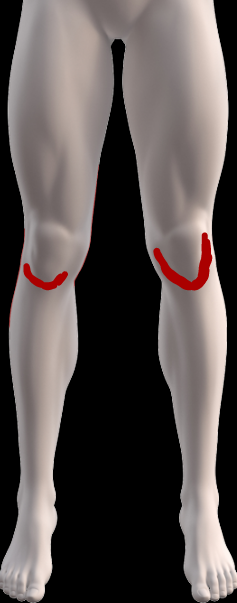
\includegraphics[width=0.25\textwidth]{figures/kneepainmap}
\caption{Pain drawings of the lower extremities. The red markings indicate the area of pain perceived by the individual subject. In this case the PFP is bilateral (on both knees).}
\label{fig:kneepainmap}
\end{figure}

\subsection{Navigate Pain}
Navigate Pain is an application that is used to visualise the location, shape and spatial distribution of pain from patient to healthcare personnel. The application permits subjects to draw their pain into a body outline with different colors and line thickness. Navigate Pain is developed by Algance Solutions within Aalborg University in Denmark.\citep{Solutions2015}
\autoref{fig:Navigatepain} illustrate the process using the application.

\begin{figure} [H]
\centering
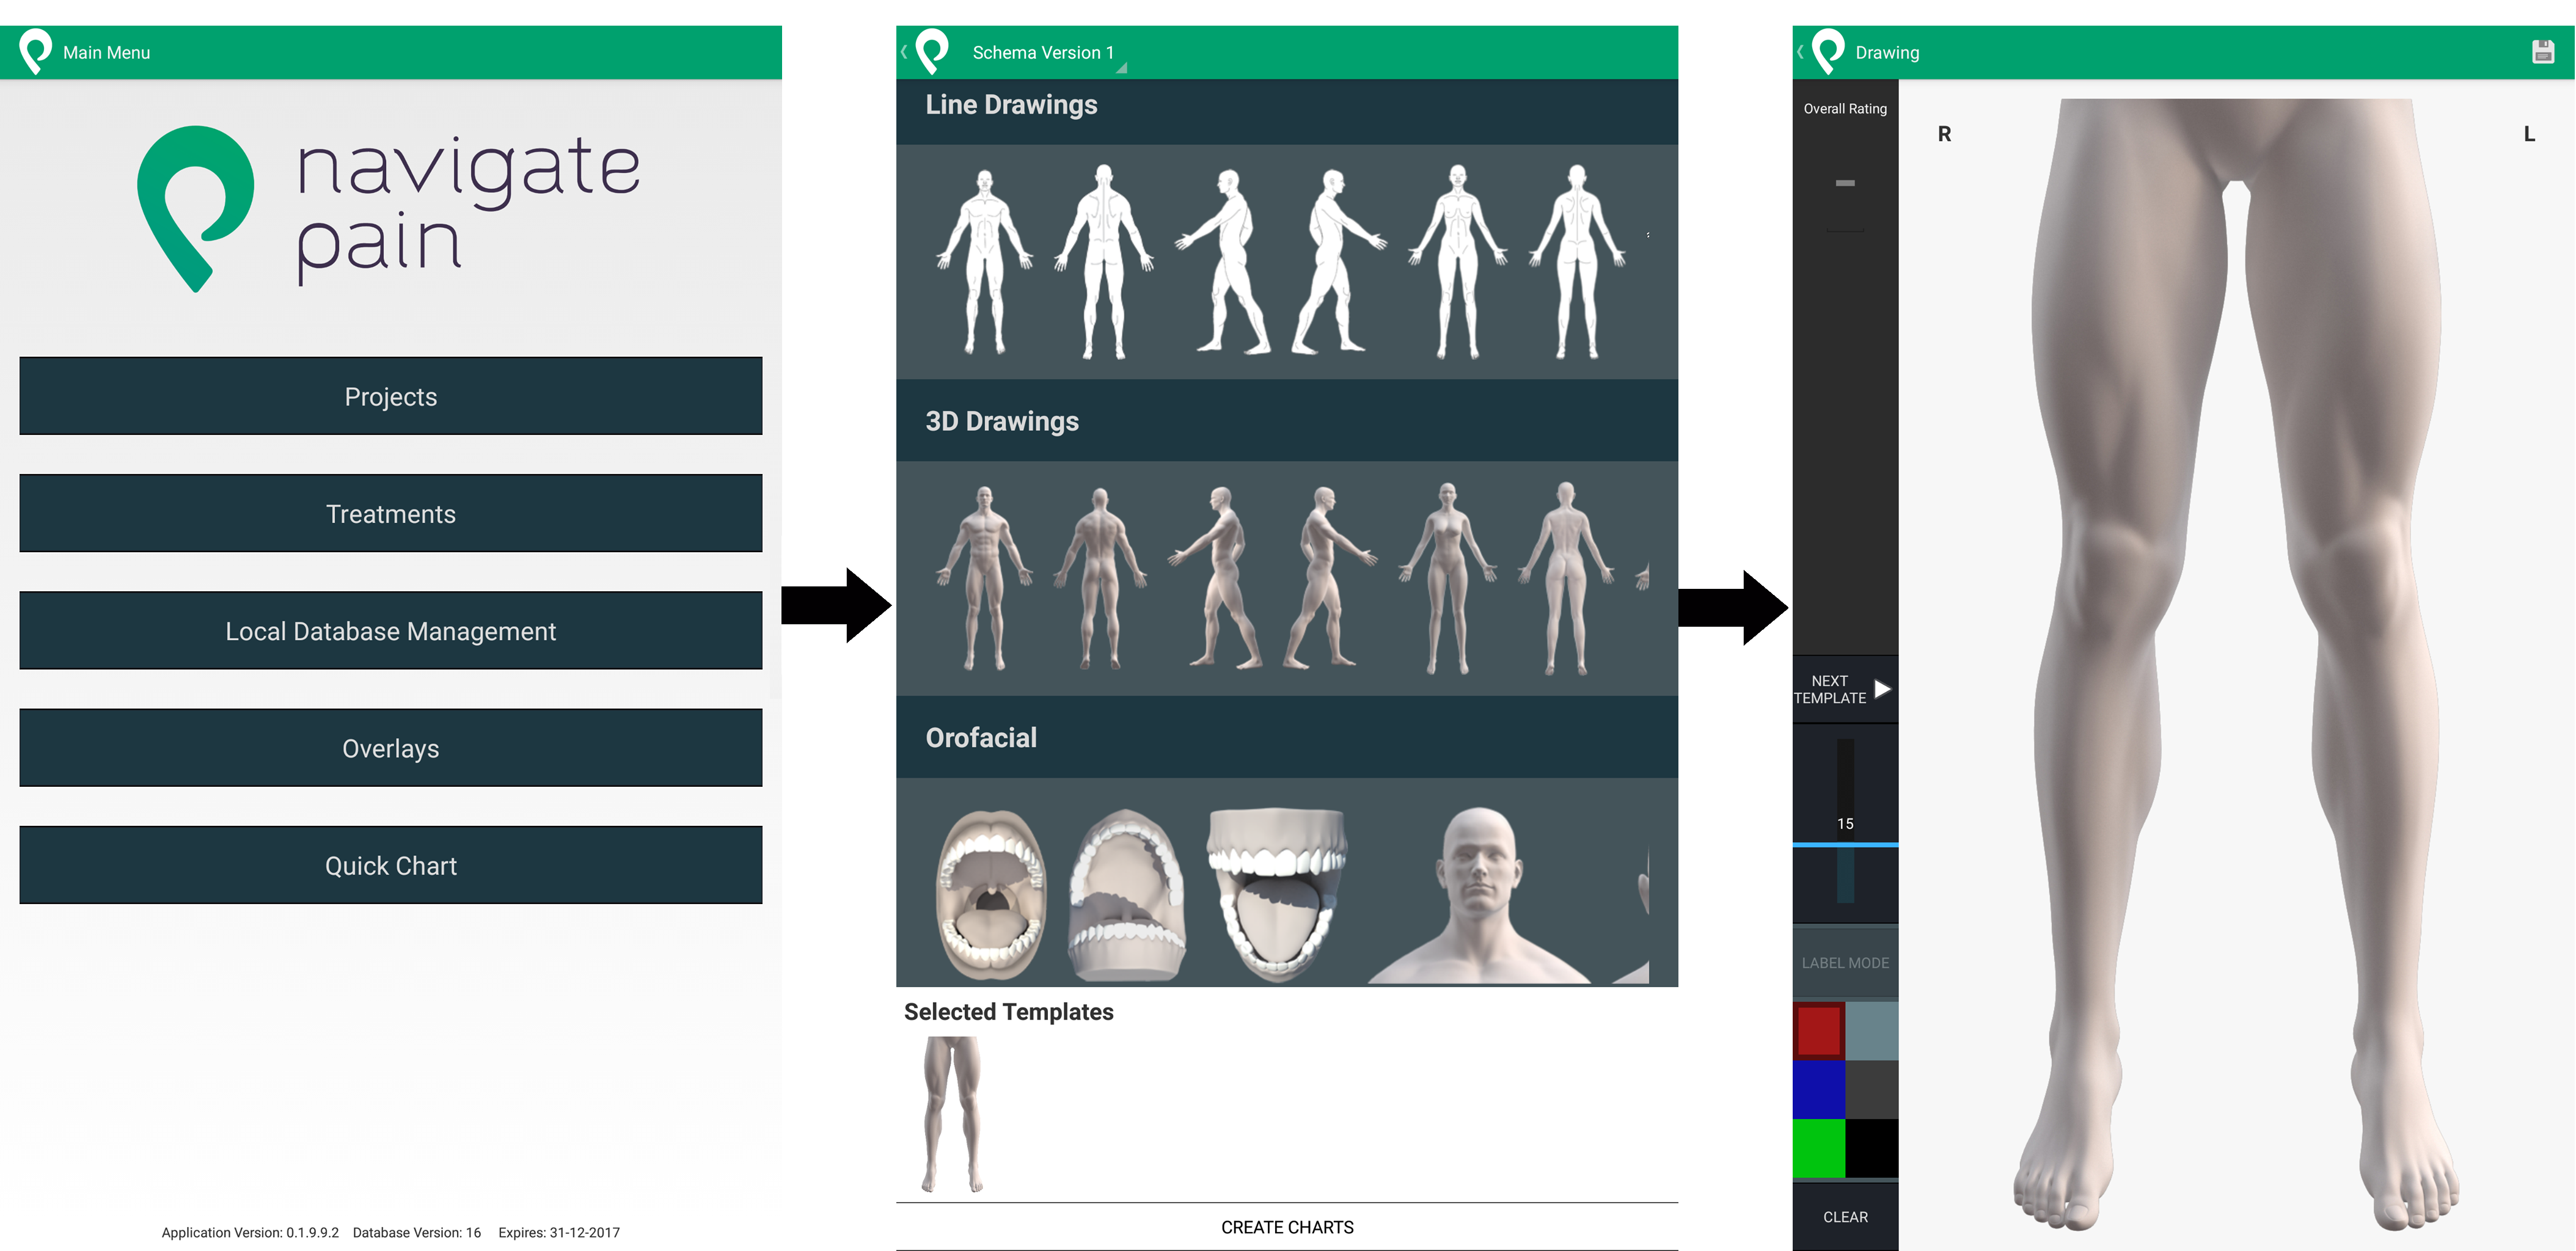
\includegraphics[width=1\textwidth]{figures/Navigatepain}
\caption{The figure illustrates the process for making a pain map with Navigate Pain. There is three screenshots of the application.}
\label{fig:Navigatepain}
\end{figure}

\noindent
The left screen in figure \ref{fig:Navigatepain} is the main screen. By clicking on "Project" a folder with subjects is created. From each subject information like name, age, height is saved. Before the subject can draw their pain areas, the body outline has to be chosen, which illustrates the screen in the middle. The body outlines is divided into five categories: Line Drawings, 3D Drawings, Orofacial, Special Zooms and Knee Pain. In the bottom the seleceted templates is shown. When clicking on "CREATE CHARTS" the right screen is shown. Here it is possible to draw the pain areas with different colors and line thickness, which can be seen in the left side of the screen. Afterwards the pain map can be saved. 
